\section{Implementation details}

    Before starting the work on this project I did a somehow similar piece of software. 
    That project gave me the idea to implement develop the project that I am currently talking about that I now write about.

    I first wanted to draw the recursive line in a SVG element, I also wanted to draw a grid for every layer. 
    The way the layers are structured in the final version was not thought from the start, it was a process of trial and error.

    The main piece of code was written in a handful of days. 
    It was written in pure JavaScript with very poor architecture. 
    It could draw lines but it was clear that the bugs and the general code repartition would not allow space for further improvements. 

    After struggling some time I decided to use a different approach.
    I decided to rewrite all of my code in CoffeeScript. I never used it or anything alike till then. 
    I had the wrong opinion that CoffeeScript would be to high-level and would hard to debug after transforming it to JavaScript. 
    This was not the case.

    CoffeeScript is a very thing layer over JavaScript.
    Most lines in CoffeeScript can be easily converted to JavaScript, without to much hassle.
    I talked about this before.

    After a day or two I, finally, managed to transform all my code to CoffeeJS.
    The didn't mean that my code got better.
    It still lacked modularity and was generally speaking - bad code.

    Using the CoffeeJS \xt{class} construct I managed to implement a better structured OOP architecture.

    \subsection{The Vector class}

        During all the geometry transformations, lots of times, I had to transform cartesian coordinates to polar coordinates and vice-versa.
        I could create two functions that would transform to and from these coordinates systems.
        But it was clear that using such an approach would be tedious.
        This problem arose at my first project (I talked about it earlier).

        I tried to resolve this by implementing a class that could store and return at the same time both types of coordinates.
        The class had 4 properties : \\
        \xt{orthX, orthY, polarRad, polarAng} 

        These were closure \cite{closures} variables so the user could not access them.
        I provided several methods for interaction, like: \\
        \xt{setX(),  getAng(), getY(), setRad()}, etc.


        Inside these functions, beside setting or returning the requested variable I would recalculate the coordinates.
        For example if a user used \xt{setAng()}, I would set the angle to the given value and, after that, would recalculate the cartesian coordinates.
        In this way, every calculation happened without the knowledge of the user.


        The problem with this was that it was still to cumbersome.
        That was when I found out about a very interesting and obscure feature of JavaScript \cite{defineProperty}.

        \subsubsection{Object.defineProperty}

            Basically this function allows to define all kinds of properties for variables. For example:
            \begin{lstlisting}
            Object.defineProperty(this, 'y', {
                get : function() {
                    return orthY;
                },
                set : function(val) {
                    orthY = val;
                    this.recalcPolar();
                }
            });
            \end{lstlisting}

            This piece of code defines a property \xt{y} that would return the private value \xt{orthY} when used, for example:
            \begin{lstlisting}
            var otherVariable = object.y;
            \end{lstlisting}
            will return the private variable \xt{orthY} from inside the closure of \xt{object}.

            This is doesn't look very useful but the \xt{get} function defines a more interesting behavior. When someone assigns a value to property \xt{y} it not only changes the variable \xt{orthY}, it also recalculates the polar coordinates. For example, the user can use \\
            \begin{lstlisting}
            object.y = 5;
            \end{lstlisting}
            instead of
            \begin{lstlisting}
            object.setY(5);
            \end{lstlisting}

            An even more interesting behavior can be observed below
            \begin{lstlisting}
            object.y += 3;
            \end{lstlisting}
            Here we increase the \xt{y} value the recalculate the points. Writing this using simple functions would look like this:
            \begin{lstlisting}
            object.setY( object.getY() + 3 );
            \end{lstlisting}

            Now the real power of \xt{Object.defineProperty()} can be observed.

    \subsection{Basic Geometry and point transformation}

        After the user moves the points on the SVG layers I needed a way to transform that location of the points to a different line. 
        One of the biggest fears that stopped me from starting to work on this project was that I was not sure how to implement the line transformations. 
        After implementing the Vector class I used a very simple technique.
        This technique will be explained below.

        \subsubsection{Simple Transformation}

            Suppose we have this setup:

            \begin{figure}[ht]
                \centering
                \caption{Initial state of the points.}
                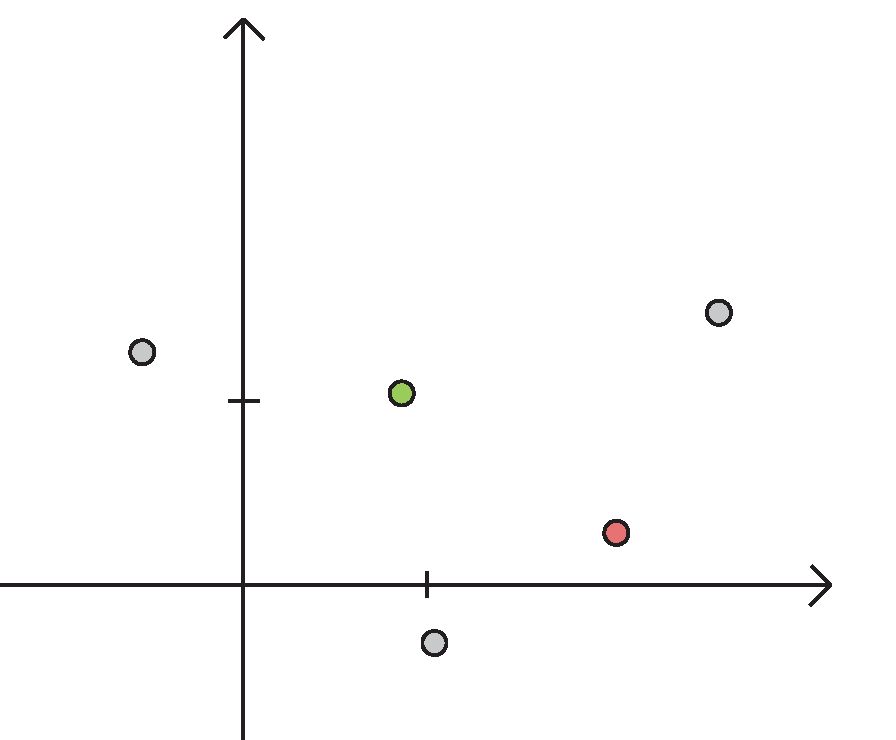
\includegraphics[scale=0.6]{img/explain01.png}
            \end{figure}

            \FloatBarrier

            We have several points. 
            The green one represents the start of the segment and the red one the end of the segment.
            I start by translating the points so that the start point coincides with the center of the coordinate system.
            At the same time I find the angle between the segment that links the start and end point and the X-axis.

            \begin{figure}[ht]
                \centering
                \caption{After translation. The angle.}
                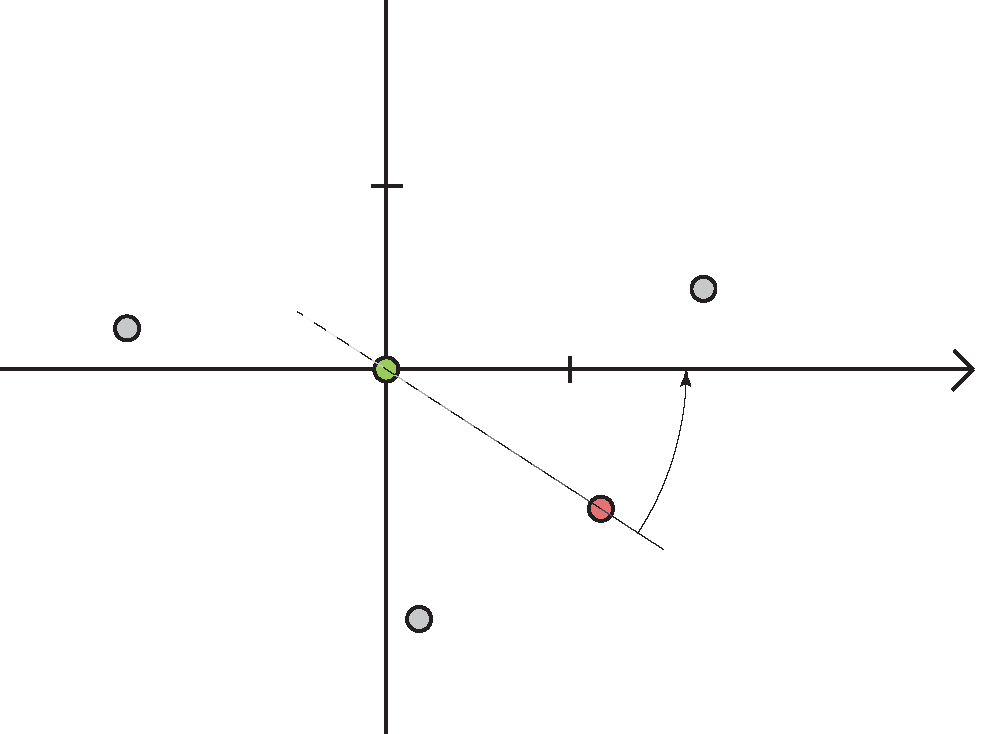
\includegraphics[scale=0.6]{img/explain02.png}
            \end{figure}

            \FloatBarrier

            Now I rotate all the points with that angle so that the end point is on the X-axis.
            All the other point follow by.

            \begin{figure}[ht]
                \centering
                \caption{After translation. The angle.}
                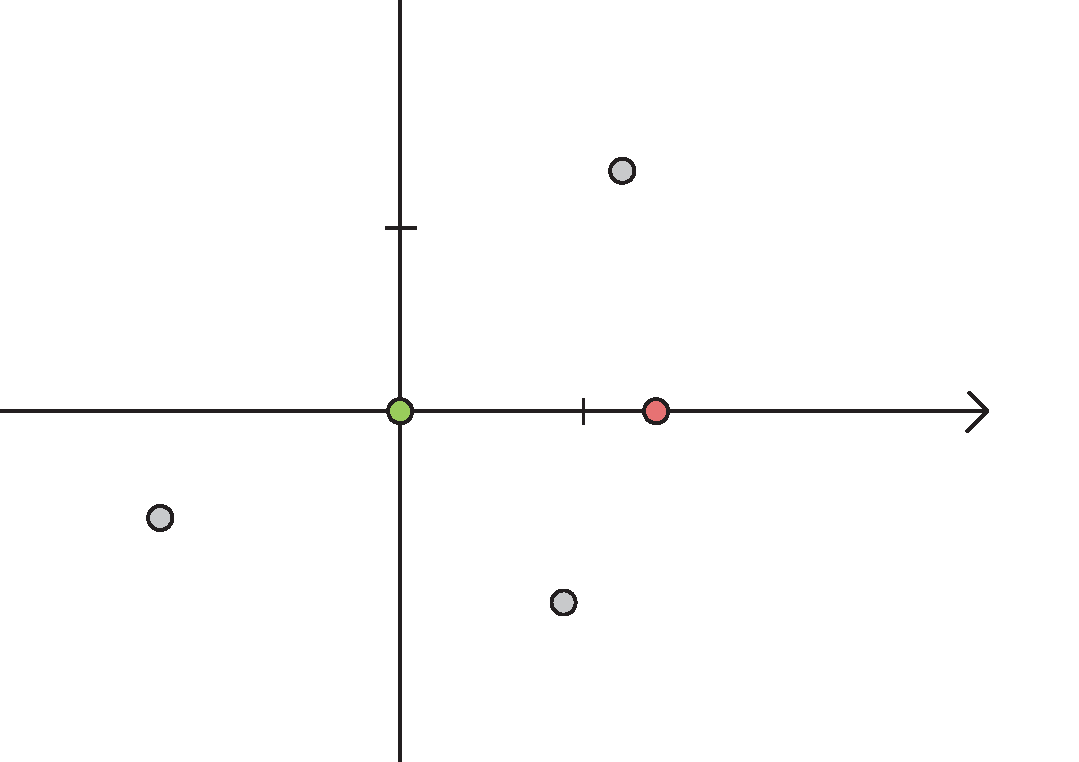
\includegraphics[scale=0.6]{img/explain04.png}
            \end{figure}

            \FloatBarrier

            Finally, I scale all the points such that the end point is on (1, 0) on cartesian coordinates.

            \begin{figure}[ht]
                \centering
                \caption{After scaling.}
                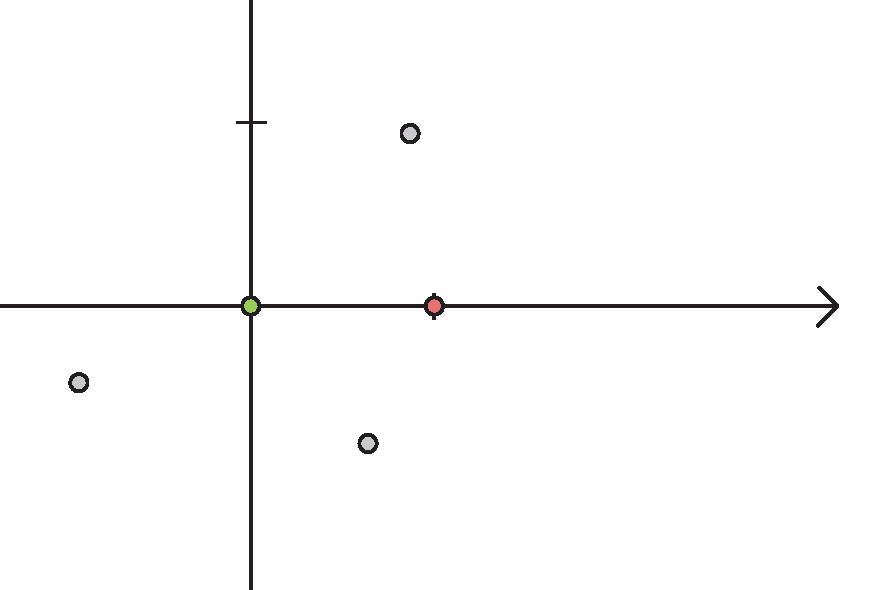
\includegraphics[scale=0.6]{img/explain05.png}
            \end{figure}

            \FloatBarrier

            In such a way the vector that connect the start point with the end point is the X-axis unit vector.

            All these transformation occur inside the function \xt{toUnitVectors()}.
            This function is called from the method \xt{getData()} of the \xt{LineLayer} class.
            Basically the user can call the method on a particular SVG layer and the layer will calculate the data and will return it in a compact form.
            Of course the function \xt{getData()} also returns data about the lines between the points but this is trivial task.

            Here is the code
            \begin{lstlisting}
    toUnitVectors: function(points){
        var ret = [];

        // There should exist at least two points
        if (!(points[1] && points[0])) return;

        // Vector from start point to end point
        var dir = new Vector(points[1].x - points[0].x, points[1].y - points[0].y);
        
        for (var i=0; i<points.length; ++i) {
            // vector from start point to point[i]
            var v = new Vector(points[i].x, points[i].y);

            // Translate the point
            v.x -= points[0].x;
            v.y -= points[0].y;

            // Change angle
            v.ang -= dir.ang;

            // Scale distance
            v.rad /= dir.rad;

            ret.push(v);
        }
        return ret;   
    }
            \end{lstlisting}


        \subsubsection{A faster algorithm}

            One might argue that it would be a better idea to implement something that would not require so much computation and storage.
            For example to use simple matrix transformations and to not use a complex data type like Vector but stick to a simple one, an array of two elements for example.
            This behavior will be probably implemented, but there are other, more important problems that need to be solved. 

    \subsection{Recursive drawing}

        Another problem that I had to tackle is choosing an optimal recursive drawing algorithm.
        The core is clear, I iterate through the segment calling the function recursively till I get to deepness 0 when I draw the line.

        If I would use this simple approach the program might resist for simple drawings but it would completely freeze if there a lot of functions.
        And I think when the number of calls gets to 300000, that can be called a lot of functions.
        Besides this, even if the program might succeed in drawing the segments the user will be unable to move anything while the program is drawing.
        That was a major drawback.

        \subsubsection{Asynchronous JavaScript}

            JavaScript is known as a language than can be easily used for asynchronous function callback.
            You give a function, give a number of milliseconds, and after that time passes the functions is executed.
            There are to basic functions that provide this functionality: \xt{setTimeout(func, millis)} and \xt{setInterval(func, millis)}.
            The first one executes the function just one time, the second executes the function indefinitely.
            The execution can be stopped by \xt{clearTimeout(timeout)} and, respectively \xt{clearInterval(interval)}.

            There are a lot of myths about these two functions.
            First of all people tend to think that JavaScript uses multiple threads to handle asynchronous functions. 
            Unfortunately it does not. 
            As I side word there start to appear some functionality in JS that would permit multi-threading.
            This, however, is beyond the scope of this paper.
            The reader might want to search for \emph{Javascript Web Workers}.

            All the asynchronous functions are executed on the same thread.
            The exact implementation varies from browser to browser but I will try to give a simplified explanation.
            First of all there is a queue that catches all the asynchronous execution, be it the main program, a function called with \xt{setTimeout()} or even \xt{XMLHttpRequest}.
            I will talk only about timeouts and intervals, and the differences between the two.

            If a timeout or an interval fires and there is nothing to be executed, the asynchronous function is just executed.
            If there is another process running the asynchronous function is queued.
            The interesting thing is that if an interval fires another time while the last occurrence was not executed, the new occurrence will be dropped.

            There are two approaches for handling iterative asynchronous function calling. 
            First there is setting up an interval.
            The second is to set up a timeout and reset that timeout inside the function that he fires.
            There is a slight difference between two approaches.
            More about this can be found in the book \emph{Secrets of the JavaScript Ninja} \cite{js_ninja}, chapter 8 \emph{Taming threads and timers}.


        \subsubsection{Asynchronous Recursive Drawing}

            With the knowledge from the previous paragraph the user might have observed a very good optimization.
            Instead of just recursively calling the function that deals with drawing the program might set a timeout.
            In that way the program will not freeze.
            It might take him a little more time but it will not freeze.

            The problem with this approach was that it is to expensive.
            There were cases when I got more than 1~GB used by the browser.

            Not only were a lot of variables declaration in every function call, also, there were a lot of functions firing at the same time.
            Imagine how was the browser feeling with more than 10 thousand timeouts firing at the same time.
            Expecting the browser to take care of the queue by himself is not what a gentleman would do.

        \subsubsection{An Asynchronous Iterative approach}

            For some it might have been clear from the beginning that the best approach would be to create a queue, pass all the data for the function in that queue and then take one element after another until the queue gets empty.
            I didn't adapt this technique from start because I was lazy.

            First of all I changed a little bit the values that were passed to the function.
            On the first variant the function would get the starting points of the segment in form of Vector points, the type of the segment and the level of the recursion.
            The most obvious optimization was to not pass a Vector object but just two numbers for every point.

            Every call to the function would populate the queue.
            From a different function I would control the execution of the queue.
            I used a timeout to execute the function.
            I soon realized that the timeout could execute the function more than one time.
            I introduced a variable that controlled how many time that function would get executed every timeout.
            Now it is set at around 300 times.
            This is a number that lets the user interact with the browser while the function is still drawing.

        \subsubsection{The last optimization}

            I observed another thing that could be optimized.
            Every function call would create some new variables. 
            Letting the JavaScript garbage collector control when the variables were disposed was not the best idea.
            Also the fact of allocating a new variable was itself time consuming.

            I decided to use function from outside the function.
            In this way every function would use the same functions, just like static functions in other languages.

            Inside the function there are cases when I allocated a new Vector object. 
            An optimization was to use the same object and only change his data.

            In this way the drawing got more fast.
